\section[Main objective]{Main objective}
\label{sec:main_objective}

The \textbf{main object} of the project is to generate a reliable \textbf{time series forecasting} based on sales from Favorita stores, which is a  grocery retail store based in Ecuador. Producing an accurate forecast could lead to decreased food waste related to overstocking and improve customer satisfaction. 

All the code can be found in the following \href{https://github.com/razielar/forecasting_retail-store}{GitHub repository}, further information can be found in \nameref{sec:supp_info}.

\clearpage

\section[Data description]{Data description}
\label{sec:data_description}

The dataset comes from \textbf{Kaggle}, named: \href{https://www.kaggle.com/competitions/store-sales-time-series-forecasting/data}{Store Sales - Time Series Forecasting}. The Kaggle dataset contains sales data from \textit{Corporación Favorita}, a large Ecuadorian-based grocery retailer. Kaggle provides you with 7 diffeent files (see \autoref{tab:files} for more details). 

\begin{table}[!htb]
  \caption[Kaggle files description]{\textbf{Kaggle files description}. Files are alphabetically sorted.}
  \begin{scriptsize}
    \begin{tabulary}{0.65\linewidth}{ccl}
      \textbf{Number} & \textbf{File Name} & \textbf{Description} \\ \hline
      1 & holiday\_events.csv & Relevant holidays in Ecuador  \\
      2 & oil.csv & Oil prices from 2013 to 2017  \\
      3 & sample\_submission.csv & submission example  \\
      4 & stores.csv & Stores metadata  \\
      5 & test.csv & Stores and family products  \\
      6 & train.csv & Sales by store and product-family from 2013-01 to 2017-08  \\
      7 & transactions.csv & Number of transactions by store  \\
    \end{tabulary}
  \end{scriptsize}
  \label{tab:files}
\end{table}

The training data represents 99\% of the data, including dates from 2013-01-01 to 2017-08-16 (55.5 months), 54 stores placed in different cities within Ecuador, and 33 family-products (see \autoref{fig:store_summary}). The testing data includes dates from 2017-08-16 to 2017-08-31 (15 days).

\begin{figure}[!htb]
  \centering
  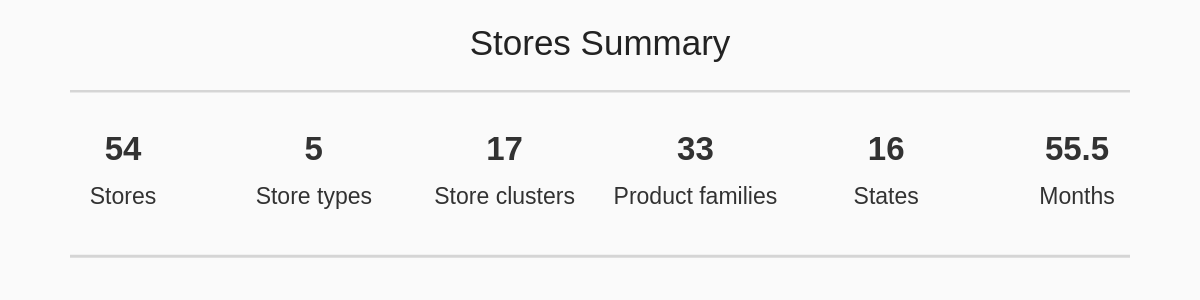
\includegraphics[width=0.9\textwidth]{plots/data_description/stores_summary.png}
  \caption[Summary of the training dataset]{\textbf{Summary of the training dataset}. The cluster information denotes similarity between stores.}
  \label{fig:store_summary}
\end{figure}

\section[Data exploration and data cleaning]{Data exploration and data cleaning}
\label{sec:eda}

Performing an exploratory data analysis (eda) of the sales from the training dataset, we can observe that grocery I, beverages, and produce are the top 3 most consumed products (see \autoref{fig:eda}) . Additionally, store type A, and cluster 5 are the most frequent among their classification.

\begin{figure}[!htb]
  \centering
  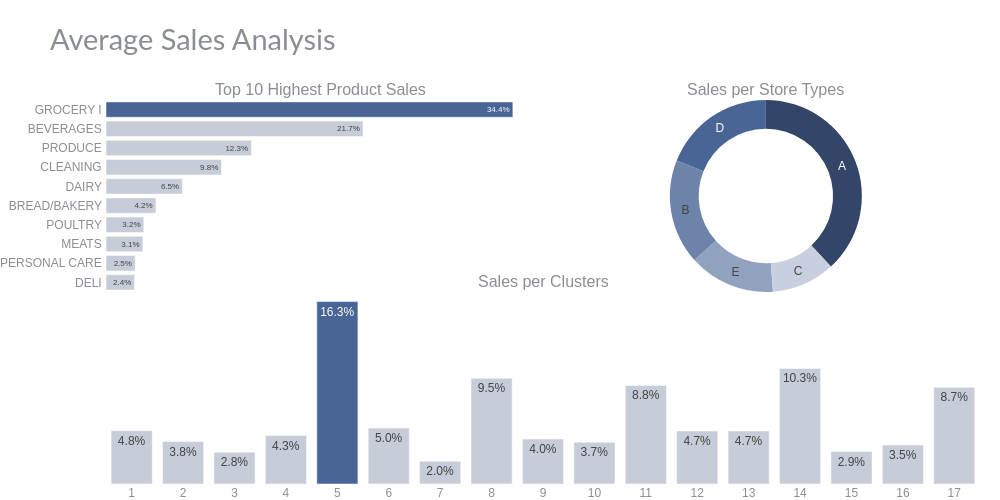
\includegraphics[width=0.9\textwidth]{plots/eda/sale_analysis.png}
  \caption[EDA of sales]{\textbf{EDA of sales}. The plot describes the sales by product, store type, and per cluster (left, right, and below, respectively). Darker blue represents higher sales. }
  \label{fig:eda}
\end{figure}

\subsection[Stationarity and seasonality analyses]{Stationarity and seasonality analyses}
\label{sec:st_s_analysis}

\begin{figure}[!htb]
  \centering
  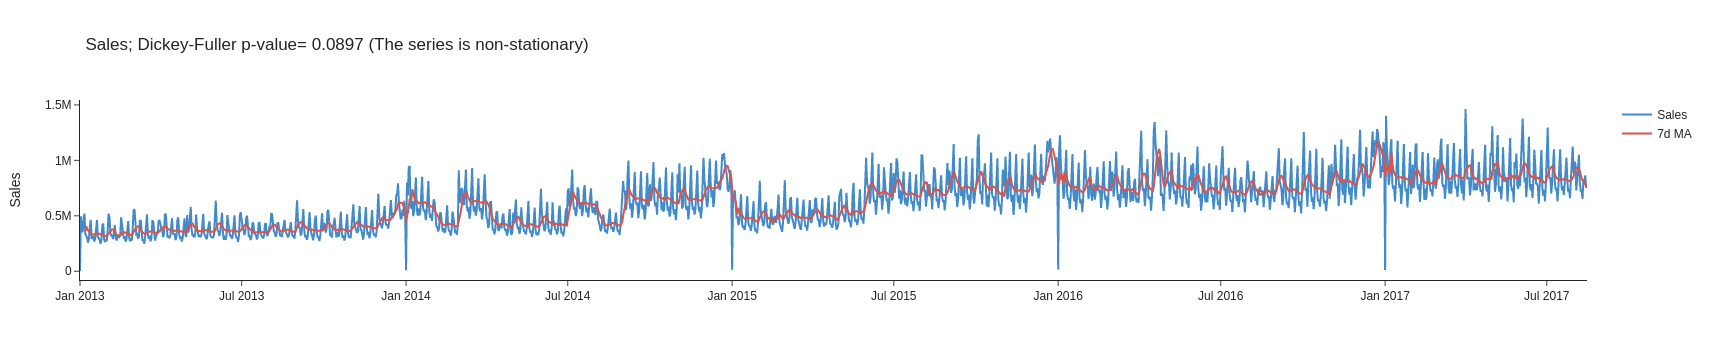
\includegraphics[width=1\textwidth]{plots/eda/target-time-series-plot-DF-test.png}
  \caption[EDA of sales]{\textbf{EDA of sales}. The plot describes the sales by product, store type, and per cluster (left, right, and below, respectively). Darker blue represents higher sales. }
  \label{fig:eda}
\end{figure}

